\chapter{Recurrence Relations}
\begin{stbox}{General Information}{}
  \begin{enumerate}
    \item Solving RRs in general:
    \begin{enumerate}
      \item Continually expand \(u_n\) in terms of \(u_{n-1}\), then in terms of \(u_{n-2}\), and so on, till an explicit formula is obtained.
      \item Alternatively, start from \(a_1\) and iteratively find \(a_2\), \(a_3\), \ldots, \(a_n\).
    \end{enumerate}
    \item Solving \(u_{n+1}=au_{n}+b\):
    \begin{enumerate}
      \item Iteration --- Apply 4(a) and use the geometric sum formula.
      \item
      \begin{enumerate}
        \item Rewrite the RR as as \(u_n-k=a(u_{n-1}-k)\), where \(k=\frac{b}{1-a}\). Let \(v_n=u_n-k\).
        \item Then, show that \(a=\frac{v_n}{v_{n-1}}\) is a constant, so that \(\{v_n\}\) is a geometric progression with first term \(v_1-k\) and common ratio \(a\). 
        \item Now, \(v_n=(u_1-k)a^{n-1}\) and \(u_n=v_n+k=(u_1-k)a^{n-1}+k\).
      \end{enumerate}
      \item \(\bigstar\) Let \(u_n=Aa^n+\frac{b}{1-a}\) and solve for the constant \(A\) using the initial conditions provided.
    \end{enumerate}
    \item Solving \(u_{n+2}=au_{n+1}+bu_n\):
    \begin{enumerate}[label=\roman*.]
      \item The characteristic equation is \(\lambda^2-a\lambda-b=0\), which has roots \(\lambda_1\) and \(\lambda_2\).
      \item The general solution is
      \[u_n=\begin{cases}
        (An+B)\lambda^n &\text{if \(\lambda=\lambda_1=\lambda_2\)},\\
        A\lambda_1^n+B\lambda_2^n &\text{if \(\lambda_1\neq\lambda_2\)},\\
        r^n[A\cos(n\theta)+B\sin(n\theta)] &\text{if \(\lambda_1=re^{i\theta}\) and \(\lambda_2=re^{-i\theta}\) are not real},
      \end{cases}\]
      where \(A\) and \(B\) are real constants. \emph{Note.} Even if \(\lambda_1\) and \(\lambda_2\) are complex, \(u_n=A\lambda_1^n+B\lambda_2^n\) is valid.
      \item Solve for the constants \(A\) and \(B\) using the initial conditions provided.
    \end{enumerate}
  \end{enumerate}
\end{stbox}
\begin{note}\hypertarget{vieta}{}
  We should remember Vieta's Formula. Consider a complex polynomial \(a_2 z^2+a_1 z+a_0\) with roots \(r_1\) and \(r_2\). Then, the sum \(r_1+r_2=-a_1/a_2\) and the product \(r_1r_2=a_0/a_2\).
\end{note}
\begin{note}
  Let \(x_{n+1}=f(x_n)\) and \(L\coloneq \lim{x_n}\). To find the possible values of \(L\), we can compare the graph of \(y=f(x)\) against the identity function \(y=x\). This is done by seeing if \(f(x)<x\), \(f(x)=x\), or \(f(x)>x\).
\end{note}
\begin{example}{}{}
  \begin{figure}[H]
    \centering
    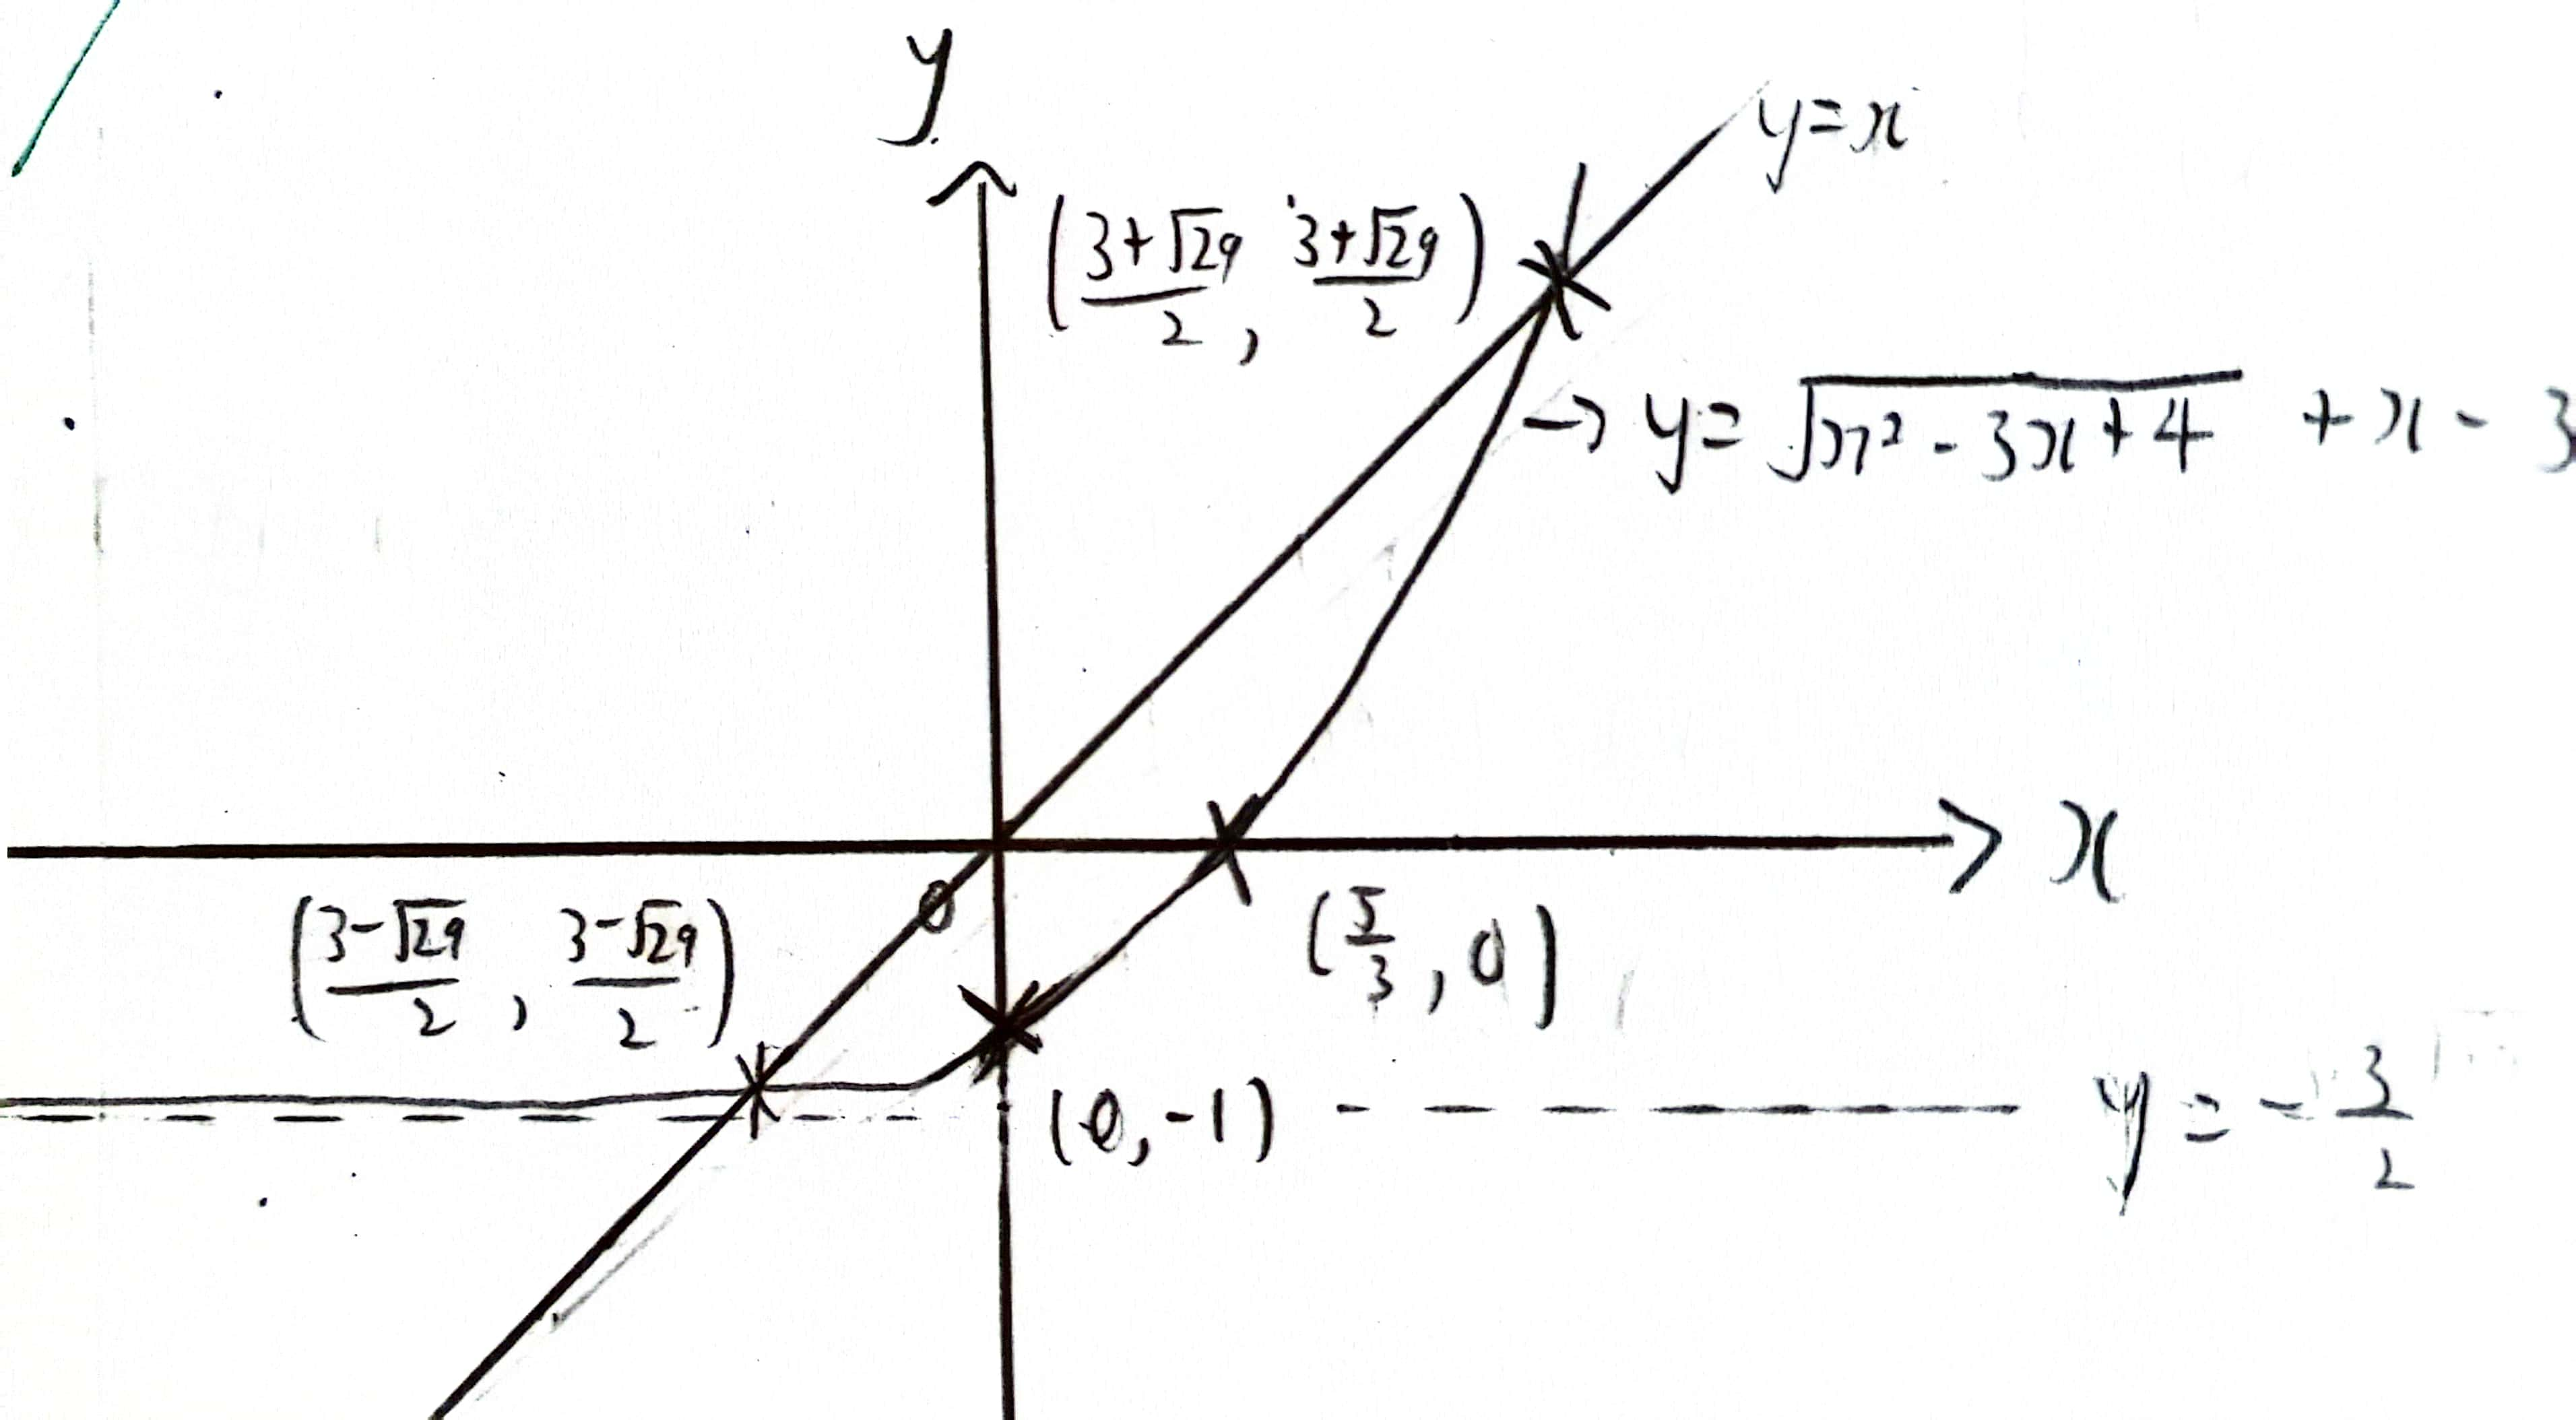
\includegraphics[scale=0.05]{SpecialRR.jpg}
    \caption{\ref{Me} The RR \(x_{n+1}=\sqrt{x_n^2-3x_n+4}+x_n-3\).}
    \label{fig:RR-identiy-function-comparison}
  \end{figure}
  \begin{center}
  \end{center}
  Let \(f(x)=\sqrt{x^2-3x+4}+x-3\).
  \begin{enumerate}
    \item Suppose \(x_1 \leq \frac{3+\sqrt{29}}{2}\). For \(x_1<\frac{3-\sqrt{29}}{2}\), we see that \(f(x)>x\). So \(x_n\) increases till \(\frac{3-\sqrt{29}}{2}\). In contrast, for \(\frac{3-\sqrt{29}}{2}<x_1<\frac{3+\sqrt{29}}{2}\), we have \(f(x)<x\). Thus \(x_n\) decreases till \(\frac{3-\sqrt{29}}{2}\). Notice the graphs intersects at \(x=\frac{3-\sqrt{29}}{2}\). This suggests that \(L=\frac{3-\sqrt{29}}{2}\).
    \item Similarly, if \(x_1=\frac{3+\sqrt{29}}{2}\), then \(x_n=\frac{3+\sqrt{29}}{2}\) is a constant function; \(L=\frac{3+\sqrt{29}}{2}\).
    \item Presume that \(x_n>\frac{3+\sqrt{29}}{2}\). Then, \(f(x)>x\) tells us \(x_n\) is an increasing sequence that is unbounded. In other words, \(L\) does not exist.
  \end{enumerate}
\end{example}
\begin{note}
  When we are asked to comment on the proposed model, it is usually about how suitable it is in modelling the actual situation.
\end{note}
\begin{example}{}{}
  Investigate what the model, with these values of \(a\) and \(b\), predict about the population when \(M_0=9679\) and \(M_0=9681\), respectively. 
  \begin{enumerate}
    \item[\textcolor{green!70!black}{\checkmark}] The model predicts that the population oscillates between  approximately 2420 and 9680 for the first few values of \(n\), but eventually becomes negative at \(n=9\) and \(n=10\). Hence the proposed model is valid only for the first few years and not in the long run. 
    \item[\textcolor{red}{\(\times\)}] The proposed model is very sensitive to small changes in the initial population of the mammal. 
  \end{enumerate}
\end{example}